% ============================================
% CONTOUR TEST GENERATOR - DIAGRAM SNIPPETS
% ============================================
% Copy and paste these TikZ snippets into your test

% --------------------------------------------
% NUMBER LINE (for inequalities)
% --------------------------------------------

% Basic number line
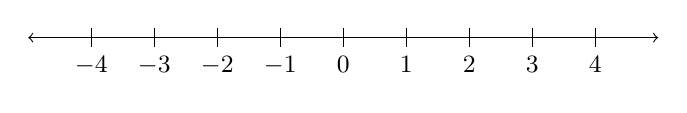
\begin{tikzpicture}[scale=0.8]
\draw[<->] (-5,0) -- (5,0);
\foreach \x in {-4,-3,-2,-1,0,1,2,3,4}
    \draw (\x,0.15) -- (\x,-0.15) node[below] {\small $\x$};
\end{tikzpicture}

% Number line with open circle (x > a), arrow right
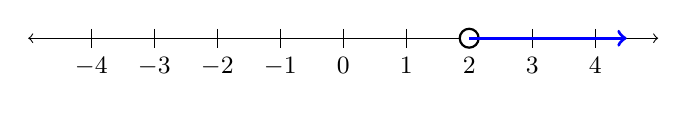
\begin{tikzpicture}[scale=0.8]
\draw[<->] (-5,0) -- (5,0);
\foreach \x in {-4,-3,-2,-1,0,1,2,3,4}
    \draw (\x,0.15) -- (\x,-0.15) node[below] {\small $\x$};
\draw[fill=white, thick] (2,0) circle (0.15);  % open circle at x=2
\draw[->, very thick, blue] (2,0) -- (4.5,0);   % arrow right
\end{tikzpicture}

% Number line with closed circle (x <= a), arrow left
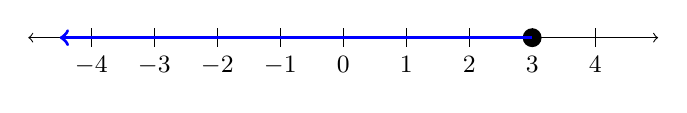
\begin{tikzpicture}[scale=0.8]
\draw[<->] (-5,0) -- (5,0);
\foreach \x in {-4,-3,-2,-1,0,1,2,3,4}
    \draw (\x,0.15) -- (\x,-0.15) node[below] {\small $\x$};
\fill (3,0) circle (0.15);                      % closed circle at x=3
\draw[->, very thick, blue] (3,0) -- (-4.5,0);  % arrow left
\end{tikzpicture}

% --------------------------------------------
% COORDINATE GRID (for graphing)
% --------------------------------------------

% Basic coordinate grid
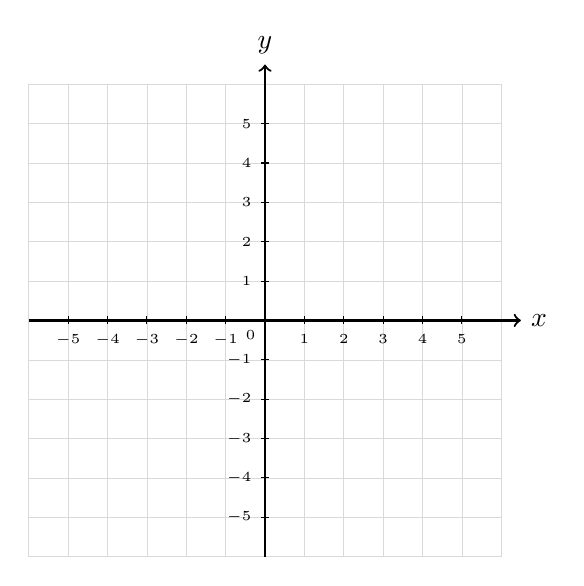
\begin{tikzpicture}[scale=0.5]
\draw[gray!30, very thin] (-6,-6) grid (6,6);
\draw[->, thick] (-6,0) -- (6.5,0) node[right] {$x$};
\draw[->, thick] (0,-6) -- (0,6.5) node[above] {$y$};
\foreach \x in {-5,-4,-3,-2,-1,1,2,3,4,5}
    \draw (\x,0.1) -- (\x,-0.1) node[below] {\tiny $\x$};
\foreach \y in {-5,-4,-3,-2,-1,1,2,3,4,5}
    \draw (0.1,\y) -- (-0.1,\y) node[left] {\tiny $\y$};
\node[below left] at (0,0) {\tiny $0$};
\end{tikzpicture}

% Two intersecting lines
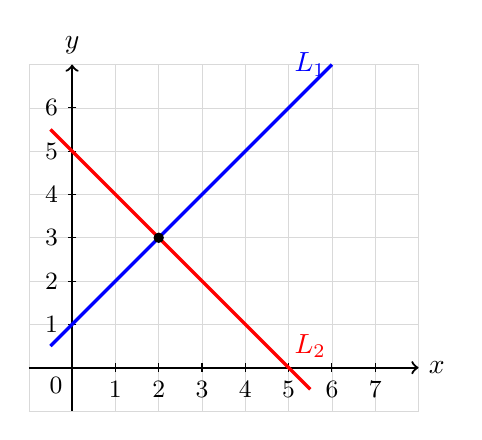
\begin{tikzpicture}[scale=0.55]
\draw[gray!30, very thin] (-1,-1) grid (8,7);
\draw[->, thick] (-1,0) -- (8,0) node[right] {$x$};
\draw[->, thick] (0,-1) -- (0,7) node[above] {$y$};
\foreach \x in {1,2,3,4,5,6,7}
    \draw (\x,0.1) -- (\x,-0.1) node[below] {\small $\x$};
\foreach \y in {1,2,3,4,5,6}
    \draw (0.1,\y) -- (-0.1,\y) node[left] {\small $\y$};
\node[below left] at (0,0) {\small $0$};
% Line 1: y = x + 1
\draw[blue, very thick] (-0.5,0.5) -- (6,7);
\node[blue] at (5.5,7) {$L_1$};
% Line 2: y = -x + 5
\draw[red, very thick] (-0.5,5.5) -- (5.5,-0.5);
\node[red] at (5.5,0.5) {$L_2$};
% Intersection point
\fill (2,3) circle (0.12);
\end{tikzpicture}

% Empty axes for student sketching (cost/distance style)
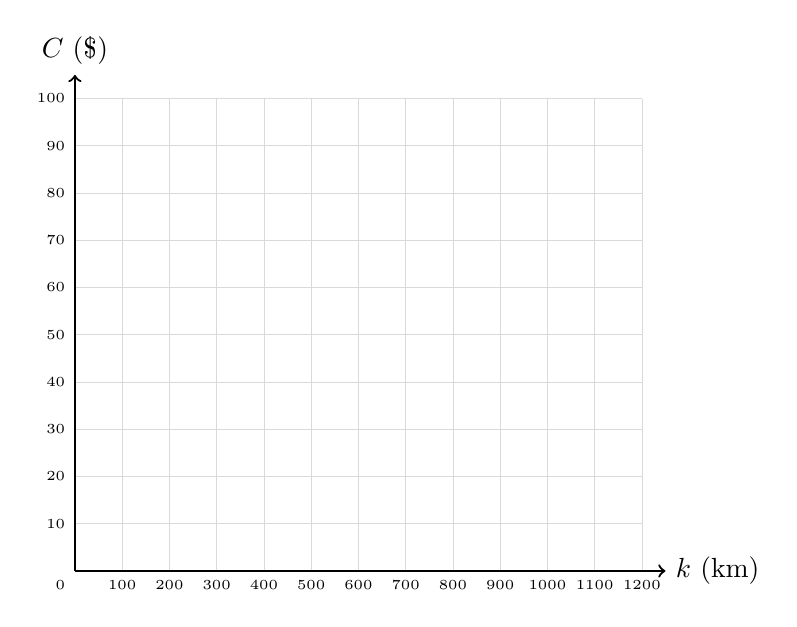
\begin{tikzpicture}[scale=0.6]
\draw[gray!30, very thin] (0,0) grid (12,10);
\draw[->, thick] (0,0) -- (12.5,0) node[right] {$k$ (km)};
\draw[->, thick] (0,0) -- (0,10.5) node[above] {$C$ (\$)};
\foreach \x in {1,2,3,4,5,6,7,8,9,10,11,12}
    \node[below] at (\x,0) {\tiny $\x00$};
\foreach \y in {1,2,3,4,5,6,7,8,9,10}
    \node[left] at (0,\y) {\tiny $\y0$};
\node[below left] at (0,0) {\tiny $0$};
\end{tikzpicture}

% --------------------------------------------
% RECTANGLE (with algebraic dimensions)
% --------------------------------------------

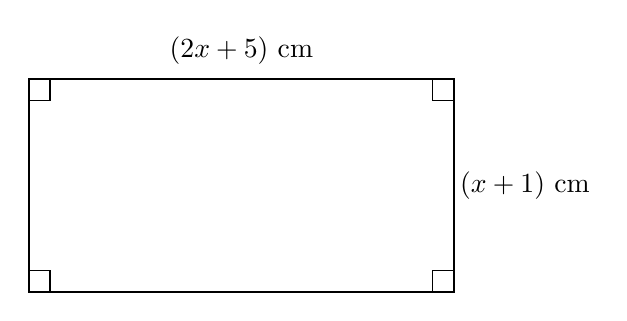
\begin{tikzpicture}[scale=0.9]
\draw[thick] (0,0) rectangle (6,3);
\node at (3,3.4) {$(2x + 5)$ cm};
\node at (7,1.5) {$(x + 1)$ cm};
% Right angle marks
\draw (0.3,0) -- (0.3,0.3) -- (0,0.3);
\draw (5.7,0) -- (5.7,0.3) -- (6,0.3);
\draw (0.3,3) -- (0.3,2.7) -- (0,2.7);
\draw (5.7,3) -- (5.7,2.7) -- (6,2.7);
\end{tikzpicture}

% --------------------------------------------
% TRIANGLE (isosceles with labels)
% --------------------------------------------

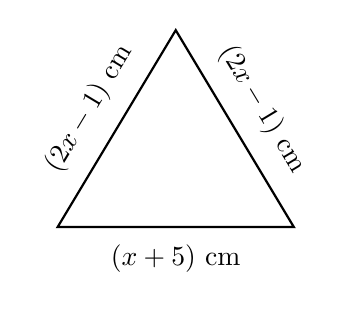
\begin{tikzpicture}[scale=1]
\draw[thick] (0,0) -- (3,0) -- (1.5,2.5) -- cycle;
\node at (1.5,-0.4) {$(x + 5)$ cm};
\node[rotate=59] at (0.4,1.5) {$(2x - 1)$ cm};
\node[rotate=-59] at (2.6,1.5) {$(2x - 1)$ cm};
\end{tikzpicture}

% --------------------------------------------
% PADDOCK/FENCING DIAGRAM
% --------------------------------------------

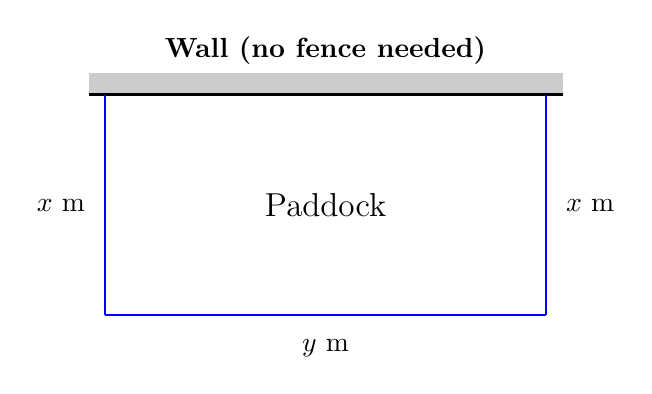
\begin{tikzpicture}[scale=0.7]
% Wall
\fill[gray!40] (-0.3,0) rectangle (8.3,0.4);
\draw[very thick] (-0.3,0) -- (8.3,0);
\node at (4,0.8) {\textbf{Wall (no fence needed)}};
% Rectangle (fenced sides)
\draw[thick, blue] (0,0) -- (0,-4);
\draw[thick, blue] (0,-4) -- (8,-4);
\draw[thick, blue] (8,-4) -- (8,0);
% Labels
\node at (-0.8,-2) {$x$ m};
\node at (8.8,-2) {$x$ m};
\node at (4,-4.6) {$y$ m};
% Area label
\node at (4,-2) {\large Paddock};
\end{tikzpicture}

% --------------------------------------------
% CIRCLE DIAGRAM
% --------------------------------------------

% Basic circle with center and radius
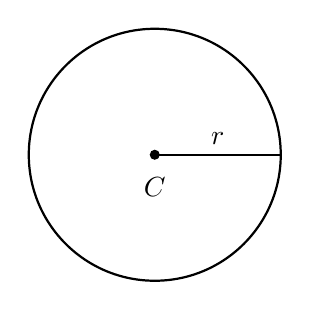
\begin{tikzpicture}[scale=0.8]
\draw[thick] (0,0) circle (2);
\fill (0,0) circle (0.08);
\node[below] at (0,-0.2) {$C$};
\draw[thick] (0,0) -- (2,0);
\node[above] at (1,0) {$r$};
\end{tikzpicture}

% Circle with tangent line
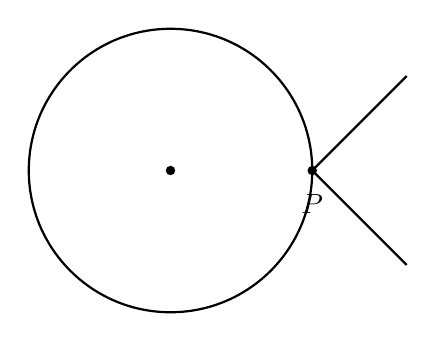
\begin{tikzpicture}[scale=0.6]
\draw[thick] (0,0) circle (3);
\fill (0,0) circle (0.1);
\draw[thick] (3,0) -- (5,2);
\draw[thick] (3,0) -- (5,-2);
\fill (3,0) circle (0.1);
\node[below] at (3,-0.3) {$P$};
\end{tikzpicture}

% --------------------------------------------
% 3D SHAPES
% --------------------------------------------

% Rectangular prism
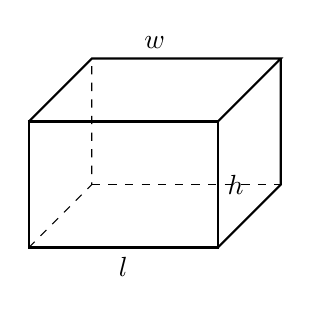
\begin{tikzpicture}[scale=0.8]
\draw[thick] (0,0) -- (3,0) -- (3,2) -- (0,2) -- cycle;
\draw[thick] (0,2) -- (1,3) -- (4,3) -- (3,2);
\draw[thick] (3,0) -- (4,1) -- (4,3);
\draw[dashed] (0,0) -- (1,1) -- (1,3);
\draw[dashed] (1,1) -- (4,1);
\node[below] at (1.5,0) {$l$};
\node[right] at (3,1) {$h$};
\node[above] at (2,3) {$w$};
\end{tikzpicture}

% Cylinder
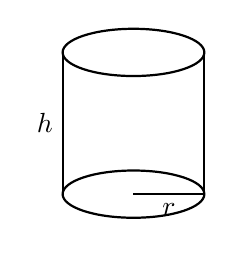
\begin{tikzpicture}[scale=0.6]
\draw[thick] (0,0) ellipse (1.5 and 0.5);
\draw[thick] (-1.5,0) -- (-1.5,-3);
\draw[thick] (1.5,0) -- (1.5,-3);
\draw[thick] (0,-3) ellipse (1.5 and 0.5);
\node[left] at (-1.5,-1.5) {$h$};
\draw[thick] (0,-3) -- (1.5,-3);
\node[below] at (0.75,-3) {$r$};
\end{tikzpicture}

% --------------------------------------------
% STATISTICAL DISPLAYS
% --------------------------------------------

% Box plot template
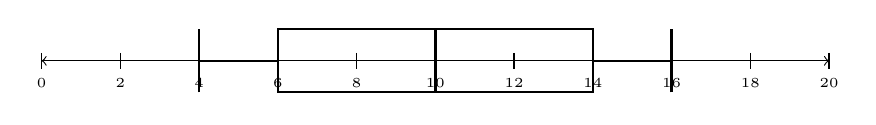
\begin{tikzpicture}[scale=0.5]
\draw[<->] (0,0) -- (20,0);
\foreach \x in {0,2,4,6,8,10,12,14,16,18,20}
    \draw (\x,0.2) -- (\x,-0.2) node[below] {\tiny \x};
% Box plot elements (adjust values as needed)
\draw[thick] (4,-0.8) -- (4,0.8);           % min whisker
\draw[thick] (4,0) -- (6,0);                % left whisker line
\draw[thick] (6,-0.8) rectangle (14,0.8);   % box
\draw[very thick] (10,-0.8) -- (10,0.8);    % median
\draw[thick] (14,0) -- (16,0);              % right whisker line
\draw[thick] (16,-0.8) -- (16,0.8);         % max whisker
\end{tikzpicture}

% Scatter plot axes
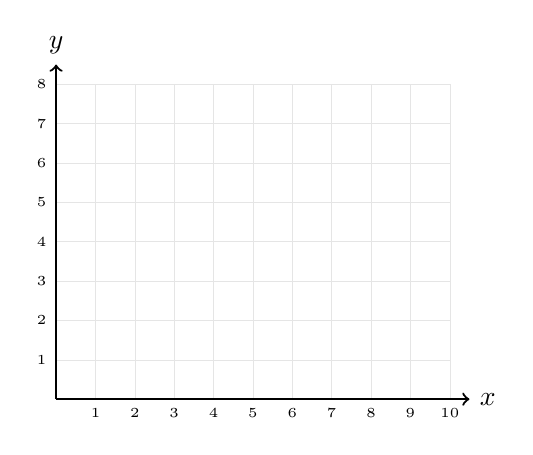
\begin{tikzpicture}[scale=0.5]
\draw[gray!20, very thin] (0,0) grid (10,8);
\draw[->, thick] (0,0) -- (10.5,0) node[right] {$x$};
\draw[->, thick] (0,0) -- (0,8.5) node[above] {$y$};
\foreach \x in {1,2,3,4,5,6,7,8,9,10}
    \node[below] at (\x,0) {\tiny \x};
\foreach \y in {1,2,3,4,5,6,7,8}
    \node[left] at (0,\y) {\tiny \y};
\end{tikzpicture}
